\documentclass[a4paper,12pt,oneside]{jsarticle}

% \usepackage{document}
\usepackage{caption}
\usepackage[dvipdfmx]{graphicx}
% \setcounter{secnumdepth}{3}



\begin{document}
% \documentclass[a4paper,12pt,oneside]{jsarticle}

% \usepackage{docmute}
% \usepackage{caption}
% \usepackage[subrefformat=parens]{subcaption}
% \captionsetup{compatibility=false}
% \captionsetup[subfigure]{labelformat=simple}
% \renewcommand{\thesubfigure}{$\left(\alph{subfigure}\right)$}
% % \renewcommand{\figurename}{Fig. }	%Fig. X yyyyyyyy と表示されるようになる

% % \renewcommand{\tablename}{Table }	%Table X yyyyyyyy と表示されるようになる
% % \captiondelim{ }

% % 以下の片方は必ずコメント化する
% \usepackage[dvipdfmx]{graphicx} %PDFを作成する場合コメント解除
% % \usepackage{graphicx}             %dviを表示する場合コメント解除 コメント解除しても見れない場合もある.解決法が見つかっていない.PDF化は問題ないので保留

% \usepackage{here}

% \graphicspath{{./graph/}}

% \begin{document}

\begin{center}
		{\Large
		2025年 部内大会
		}
	\end{center}
	\begin{center}
		\vspace*{100truept}
		{\fontsize{22pt} {0cm}\selectfont ルールブック}\\ % タイトル
		\vspace{30truept}
	\end{center}
	\begin{center}
		\vspace{170truept}	
		\vspace{15truept}	
		{\LARGE 東京農工大学 }
		{\LARGE 航空研究会}\\ 
		\vspace{15truept}
		{\LARGE 17代\hspace{5mm}大屋 悟士}\\ % 著者
		\vspace{50truept}
		\vspace{20truept}
	\end{center}
% \end{document}
\newpage
\tableofcontents
\newpage

\section{はじめに}
本大会は航空研究会に入部した新入生が主体となって活動に参加する機会を提供することを目的として開催する.
新入生のみでチームをつくり部内大会にむけた活動を行い,航空研に定着しアクティブに活動するメンバーとなることを目標とする.
また,飛行ロボコンにエントリーする上級生にも参加してもらい,飛行ロボコンにむけた練習の機会とすることで航空研全体の技術向上を目指す.

本ルールブックは第21回全日本学生室内飛行ロボットコンテストの機体レギュレーション,飛行競技ルールをもとに作成した.
本大会の性質上,飛行ロボコンでのルール質問への回答によっては本ルールが変更されることがある.
また,ルールは競技者からのルール質問を通して作り上げていくものであるから,積極的にルール質問を活用してほしい.

\section{共通ルール:出場機体・チーム構成・審査}
\subsection{プロペラ}
回転翼・ダクトファンの総称.便宜上,本大会ではヘリコプタやオートジャイロのローターのように主として揚力の発生を目的としている回転翼も全て「プロペラ」と呼称する.
プロペラの改造および作成を行った場合については十分な強度と安全性を確保した上で審査書類に明記し,機体審査において審判員に説明すること.

\subsection{機体の設計・製作・部品}
一般に市販されている飛行機・マルチコプターその他の完成品,キットの参加は許可しない.各チームで機体を企画し設計すること.

\subsection{飛行機}
固定翼機,羽ばたき機,あるいはオートジャイロのように揚力を発生させるためのプロペラを動力駆動しない回転翼機.
\subsection{ハイブリッド機}
揚力を固定翼・動力駆動するプロペラその他の装置の組み合わせによって得ており,かつ推進用のプロペラ等を備える機体.
推力方向の変更によるVTOL機もハイブリッド機に含まれる.
ハイブリッド機は部門によらず参加できる.
\subsection{マルチコプター}
揚力を複数のプロペラによってまかなう機体とする.マルチコプター部門に参加できる.

\subsection{独立した制御ユニット}
機体装備品のうち,単独モジュールとして機体から取り外すことができる装備は,下記の条件を満たすことで「独立した制御ユニット」として扱うことができる.
\begin{itemize}
  \item 独立した制御ユニットを内包できる直方体の3辺の長さの合計が25cm以下である
  \item バッテリーおよび電動モーターを含まない
  \item 独立した制御ユニットを取り外した場合であっても,機体構造が大きく変化せず,機体側に操縦用受信機が搭載されている
\end{itemize}
ただし,センサーの駆動など飛行に直接影響のない電動モーターは審査の上認められる.
「独立した制御ユニット」は空虚重量に含まれない.

\subsection{質量}
\paragraph{空虚質量} 救援物資とともに投下されるすべての投下補助器具の質量を含む機体の総質量を指す.ただし,「独立した制御ユニット」の質量は含まない.\newline
離陸重量から救援物資を除いた質量.自動操縦装置,マルチコプターに取り付けるカメラ,カメラ専用のバッテリー(およびその付属品と認められる部品),動力用バッテリー,救援物資を機体に取り付けるための補助具は空虚重量に含まれる.
\subsubsection{一般部門}
\begin{itemize}
  \item 空虚質量が$250\mathrm{g}$以下であること
  \item 「独立した制御ユニット」を搭載した機体は,空虚質量が$220\mathrm{g}$以下であること
\end{itemize}
\subsubsection{マルチコプター部門}
空虚重量が以下の条件のいずれかを満たすこと
\begin{itemize}
  \item 動力用モーターが4発以下で独立した制御ユニットを搭載していない場合:$350\mathrm{g}$以下であること
  \item 動力用モーターが4発以下で独立した制御ユニットを搭載している場合:$250\mathrm{g}$以下であること
  \item 動力用モーターが5発以上6発以下で独立した制御ユニットを搭載していない場合:$390\mathrm{g}$以下であること
  \item 動力用モーターが5発以上6発以下で独立した制御ユニットを搭載している場合:$290\mathrm{g}$以下であること
  \item 動力用モーターが7発以上で独立した制御ユニットを搭載していない場合:$430\mathrm{g}$以下であること
  \item 動力用モーターが7発以上で独立した制御ユニットを搭載している場合:$290\mathrm{g}$以下であること
\end{itemize}
動力用モーターはホバリング時に十分な推力を発生させているものを指す.
\subsubsection{質量ペナルティ}
規定重量を満たせない機体での出場を認めるが式(\ref{eq:weightPenalty}) によるペナルティを課す.
\begin{equation}\label{eq:weightPenalty}
  質量ペナルティ = 超過質量 \times 10
\end{equation}

\subsection{救援物資}
救援物資輸送ミッションで使用する物体.
これを機体に搭載するために付属物を用いることもできるが,その付属物は救援物資より軽く,かつ投下した際に床を傷つける恐れのないものに限る.
救援物資の気密を損なうことは認められない.
また,チームメンバーは競技中に投下した救援物資に触れてはならない.
\begin{itemize}
  \item 救援物資(小)(一般部門では救援物資という)は日清食品の「チキンラーメンmini」と呼称する
  \item 救援物資(大)は日清食品の「チキンラーメン」とする.
\end{itemize}


\subsection{コール}
競技参加者が後述する指定のミッションの指定のタイミングで,レフェリーにたいして指定される用語にて,自身の行動を宣言する行為.コールは操縦者および補助者によって行われる.複数のコールがあった場合,レフェリーが聞き取れた最後のコールが有効となる.

\subsection{動力}
動力として,電動モーター,バッテリーにて駆動したプロペラ,羽ばたき機構等を使用すること.オリジナル部品の使用は禁止しないが,安全性に十分配慮すること.

\subsection{バッテリー}
\begin{itemize}
  \item セル数が2以下のLi-Poバッテリーを使用すること
  \item マルチコプター部門において耐故障制御に挑戦する場合は3セルのLi-Poバッテリーの使用を認める
  \item その他,チームからの申請により審査の上認めることがある
\end{itemize}

\subsection{操縦装置}
\begin{itemize}
  \item 技適を有する無線機を使用すること
  \item フェイルセーフ機能として,送信機-受信機間の通信が切断された際にすべての動力用モーターが停止する機能を有し,その機能を使用すること
\end{itemize}

\subsection{チーム構成}
飛行競技に参加できるチームメンバーは操縦者(1名)と補助者(4名以内)の計5名以内とする.
飛行競技以外の機体製作などに関与する人数は制限しない.

\subsection{安全性}
参加機体は以下の5項目の安全性を満たすこと
\begin{enumerate}
  \item 緊急時に確実かつ速やかに動力を停止できること
  \item 進行方向に突起物がある場合は,カバーを施すなどの安全処置を行うこと
  \item 混信や通信不良に備え,送信機-受信機間の接続が切れた場合にスロットルパワーがオフになるフェイルセーフ機能を設定すること
  \item ハンズオフ飛行中においては,瞬時に操縦者による遠隔操縦に切り替えられること
\end{enumerate}

\subsection{機体審査}
\begin{itemize}
  \item 機体の安全性を書類審査,飛行動画審査,当日機体審査にて審判員が確認する
  \item 機体は本番機と同型予備機の最大2機による参加を認める.予備機の機体審査は本番機と同一の機体審査用紙で行うが,本番機と予備機に大きな期待形状の差異が認められる場合は審議の上予備機の登録が認められない場合がある.
  \item 機体審査円滑化のため,競技者による当日機体審査手続きを推奨する
  \item 大会前に,参加予定の機体が飛行競技ルールに則り競技が行えることを,飛行動画にて審査する.参加チームは別に定める要領に従って飛行動画を提出すること.
\end{itemize}

\subsection{点数の確定}
\begin{itemize}
  \item 点数は飛行競技直後のアナウンスにて確定される.その後のチームからの申告に基づく修正は行わない.
  \item 動画その他の媒体を用いた事後判定は行わない
  \item 飛行競技中の審判および得点集計のミス等が明らかな場合,該当チームに対し再飛行の提案を行う場合がある.ただし,再飛行を行った場合には,再飛行時の点数が採用される.
  \item 一般部門における「滑空ランキング点」は一般部門の全ての競技が終了した後に加算する.
\end{itemize}

\subsection{競技時間}
\begin{itemize}
  \item 最大飛行時間を4分とする
  \item 標準飛行時間を3分とする
  \item 飛行時間を競技開始から終了までの時間とする
\end{itemize}
式(\ref{eq:timeScore})により時間点を与える.
\begin{equation}\label{eq:timeScore}
  時間点 = (標準飛行時間 - 飛行時間)\times 5
\end{equation}

\subsection{順位}
下記のように順位を決定する
\begin{enumerate}
  \item 帰還に成功したチームを上位とする
  \item メインミッションに成功したチームを上位とする
  \item ハンズオフ飛行で複数のミッションに成功したチームを上位とする
  \item 得点の高いチームを上位とする
  \item 審査員判定
\end{enumerate}
得点はすべてのミッションにおける得点と時間点,質量ペナルティの合計とする.
また,部門間で得点の調整を行う場合がある.

\section{共通ルール:飛行競技}
\subsection{飛行競技エリア}
\begin{itemize}
  \item 飛行競技エリアは「離着陸エリア」「ミッションエリア」「物資投下エリア」「マージナルエリア」からなる
  \item 飛行可能領域は飛行競技エリアの上空に限る
  \item 操縦者が立ち入りできるエリアは離着陸エリアのみとする
  \item 補助員が立ち入りできるエリアは離着陸エリアおよびマージナルエリアとする
  \item 機体が静止している場合のみ,補助員は飛行競技エリア全てに立ち入ることができる.
\end{itemize}

\subsection{離陸}
\begin{itemize}
  \item 「離陸」という語句の定義はすべてこの項に従う.ただし,一般部門における「投下救援物資回収」の「離陸」はこの限りでない・
  \item 離陸は自力滑走による離陸,あるいはカタパルト等の補助具を用いた離陸,手投げ発進のいずれかとする.
  \item 補助具は滑走路もしくはバーティポート内に設置すること
  \item マルチコプターの手投げ発進は認めない
  \item 手投げは指定の手投げエリアから発進すること
\end{itemize}

\subsection{機体回収}
\begin{itemize}
  \item 「機体回収」という語句の定義は全てこの項の記述に従う
  \item 機体回収は補助員が機体を回収し離着陸エリアに運ぶことをいう
  \item 補助員は機体が静止しているとき,飛行競技エリアに立ち入ることができる
  \item 機体回収はプロペラ(に準ずる推進装置)が停止し機体が静止した状態で行う
  \item 機体回収後は離着陸エリアの滑走路もしくはボーティポート,手投げエリアから離陸してよい
\end{itemize}

\subsection{操縦}
\begin{itemize}
  \item 操縦者の遠隔操縦にて操縦する
  \item 飛行中,操縦者は離着陸エリア内を移動してよい
  \item 補助者は立ち入り可能なエリアから操縦者に指示を送ることができる
  \item 補助者以外の人から操縦者へ指示を送ることは認めない
\end{itemize}

\subsection{ハンズオフ飛行}
\begin{itemize}
  \item 機体が操縦者の遠隔操縦を受けず,自動飛行装置を用いて自立制御飛行を行っている状態
  \item 操縦者は送信機のスティックから指を離し,操縦をしてはならない
  \item 操縦者は送信機から手を離してはならない
  \item ハンズオフ飛行中およびそれ以外の飛行中であることを機体に取り付けられた発光体(LDEなど)の変化で示すこと
  \item 審判が発光体を視認できる取り付け位置および明るさとすること
  \item ハンズオフ飛行中以外は赤色点灯とする
  \item ハンズオフ飛行中はミッションに応じて,以下のような発光色の点灯とする
  \item 水平旋回:黄緑
  \item 8の字飛行:青
  \item 上昇旋回:緑
  \item 自動物資投下:青緑
  \item 機体の誘導・自己位置推定を補助する自走しない器具(マーカー)を設置することができる
  \item マーカーはポールを含めてどこに何個設置してもよい
  \item マーカーを飛行競技エリア外に設置したい場合は事前に相談すること
  \item 機体が離着陸エリア内で静止している場合に限り,競技中のマーカーの修理を認める
\end{itemize}

\subsection{ミッションの種類}
メインミッションは競技開始と同時に開始され,終了しなければ他のミッションには挑戦できない.メインミッションの開始コールは必要ない.
サブミッションは,各サブミッションに挑戦中にほかのミッションに挑戦できない.すなわち終了条件を満たした場合にのみ次のミッションに挑戦できる.

\subsection{競技開始}
競技は離着陸エリアの滑走路もしくはバーティポート上に機体を静止させた状態で開始する.手投げ発進の場合は手投げエリアにスタンバイした状態で開始する.

\subsection{ミッションの申告}
各チームは飛行競技開始前に,実施するミッションをミッション記入用紙に記入すること.また,それぞれのミッションを実施する直前にも,確認のため再度レフェリーにコールすること.
飛行時間との兼ね合いで,ミッションを省略する場合もコールすること.飛行競技中に順序を入れ替えてもよい.

\subsection{各ミッションへの再挑戦}
コールしたミッションに失敗した場合,同ミッションについてのみ再挑戦を許可する.

\subsection{再飛行・修理}
\begin{itemize}
  \item 機体が静止した場合,「機体回収」に従って機体を回収し,「離陸」項に従って離陸することを認める
  \item 30秒以内で修理可能な軽微な損傷に対しては離着陸エリア内での修理を認める
  \item 30秒以内に修理が完了できない場合はその時点で飛行競技終了となり未帰還扱いとする
  \item 修理に際しては,持ち込んだ道具を使用してよい.ただし,接着剤等を使用する場合は汚れてもよいシートを用意しその上でのみ作業すること
  \item 競技中のバッテリーの交換は禁止する
\end{itemize}

\subsection{飛行中止・警告・失格}
以下の場合は,飛行は直ちに中止され,未帰還扱いとする.中止までに完了したミッションの得点は加算される.
\begin{itemize}
  \item 最大飛行時間内に離着陸エリアに帰還することができない場合
  \item 機体に重大な損傷を受け,飛行競技が困難と判断された場合
\end{itemize}
以下の場合は警告を与える.
警告を3回受けたチームは直ちに飛行を中止し,未帰還扱いとする
\begin{itemize}
  \item 参加者や設備などに危険を及ぼす可能性がある飛行とレフェリーが判断した場合
  \item 競技者が指定されたエリアを出た場合
  \item 競技中に操縦者および補助者以外の者から補助や指示を受けた場合
  \item 審判と接触もしくは審判を妨害する行為.このとき当該ミッションを失敗と判断する場合がある
\end{itemize}
チームメンバー以外が設営作業や競技時間中に協力することは禁止とする.違反が判明した場合,警告・失格等の措置をとる場合がある
進行状況に応じて,練習飛行,ピット作業や競技前後の作業について時間制限や内容の制限を指示する場合がある

以下の場合,飛行競技中にかかわらず直ちに失格となる
\begin{itemize}
  \item 競技フィールドや設備,備品を損傷する,または損傷しようとする行為
  \item レフェリーの警告や指示に従わない場合 
\end{itemize}


\section{ミッション(一般部門)}

\subsection{メインミッション}
\paragraph{成功条件}
\begin{itemize}
\item 物資投下エリアに救援物資を1つ投下すること
\item 離着陸エリアに静止すること
  \item ただし,メインミッション終了後でも構わない
\end{itemize}
\paragraph{終了条件}
\begin{itemize}
\item 「投下完了」をコールすること
\item 次のミッションをコールすること
\end{itemize}
\paragraph{得点}
\begin{itemize}
\item メインミッション点 = 時間点 + 投下点 + メインミッション追加点
\item 時間点 = 20×(60-計測時間)
\item 投下点 = エリア1投下点 * 個数 + エリア2投下点 * 個数 + エリア3投下点 * 個数
\item エリア1投下点 = 50
\item エリア2投下点 = 150
\item エリア3投下点 = 300
\item エリア1およびエリア2,エリア3にそれぞれ1つ以上投下舌チームにメインミッション追加点 (500点) を与える
\item 投下点は「投下完了」をコールした後に,初めて離着陸エリアに着陸静止したときの救援物資の位置で確定する
\item 計測時間は競技開始からメインミッションの終了条件を満たすまでの時間である
\end{itemize}
\paragraph{付記}
\begin{itemize}
\item エリアの詳細については図\ref{fig::plane::dropArea}を参照すること
\item 投下点はエリア1およびエリア2,エリア3に投下された救援物資のうち合計得点が高くなる最大4つを選択して計算する
\end{itemize}

\subsection{サブミッション}
自動操縦,手動操縦共通のサブミッションの一覧は以下の通り.
\begin{itemize}
\item 8の字飛行
\item 宙返り
\item 無動力滑空
\item 救援物資回収
\item 高所物資回収
\item 帰還
\end{itemize}

手動操縦専用および自動操縦専用ミッションは以下の通り.
\begin{itemize}
\item ポール旋回 (手動操縦専用ミッション)
\item 水平旋回 (ハンズオフ飛行専用ミッション)
\end{itemize}

\subsubsection{8の字飛行}
\paragraph{成功条件}
\begin{itemize}
\item 8の字飛行を行うこと(飛行軌跡が「8の字」と認められること)
\item 高度変化が十分小さいこと
\end{itemize}
\paragraph{終了条件}
\begin{itemize}
\item 次のミッションがコールされること
\item 成功条件を満たすこと
\end{itemize}
\paragraph{得点}
\begin{itemize}
\item 8の字飛行点 = 200
\end{itemize}
\subsubsection{宙返り}
\paragraph{成功条件}
\begin{itemize}
\item 軌道面が地面に対して十分に垂直な宙返りをおこなうこと
\end{itemize}
\paragraph{終了条件}
\begin{itemize}
\item 次のミッションがコールされること
\item 宙返り回数が3回に達すること
\end{itemize}
\paragraph{得点}
\begin{itemize}
\item 宙返り点 = 宙返り回数 * 150
\item 上下方向に機体が1回転して宙返り開始地点に戻ってきたら1回転成功とし,宙返り回数を加算する
\end{itemize}
\paragraph{付記}
\begin{itemize}
\item 連続しての宙返りは認めない
\end{itemize}


\subsubsection{無動力滑空}
\paragraph{成功条件}
\begin{itemize}
\item 7秒以上の滑空飛行を行うこと
\end{itemize}
\paragraph{終了条件}
\begin{itemize}
\item 次のミッションがコールされること
\item 「パワーオン」がコールされること
\item 機体が接地すること
\end{itemize}
\paragraph{得点}
\begin{itemize}
\item 無動力滑空点 = 300 + 50*(滑空時間-10)
\item 滑空時間は「パワーオフ」のコールから「パワーオン」のコールまでの時間とする
\item 滑空時間の上限は20秒とする
\end{itemize}
\paragraph{付記}
\begin{itemize}
\item 「パワーオン」のコール後に動力飛行をすること
\end{itemize}
\subsubsection{救援物資回収}
\paragraph{成功条件}
\begin{itemize}
\item 他のミッションで物資投下エリアに投下した救援物資のうち1つを、機体に手を
触れない状態で回収し、離着陸エリアに着陸静止すること
  \item 機体が着陸静止した際に救援物資が離着陸エリア内にあれば、着陸の衝撃等で外れても成功とみなす
\end{itemize}
\paragraph{終了条件}
\begin{itemize}
\item 次のミッションがコールされること
  \item ただし,「帰還」を除く
\item 物資投下エリアの救援物資がなくなること
\end{itemize}
\paragraph{得点}
\begin{itemize}
\item 物資回収点 = 回収点+着陸点
\item 回収点と着陸点はともに500点とする
\end{itemize}
\paragraph{付記}
地上走行中に得点エリア外に接地した場合は離着陸エリアからやり直しとする.救援物資を回収した状態であれば,その救援物資は使用不可とする.

\subsubsection{高所物資回収}
\paragraph{成功条件}
\begin{itemize}
\item 指定された場所に設置した救援物資を回収すること
\end{itemize}
\paragraph{終了条件}
\begin{itemize}
\item 次のミッションがコールされること
\end{itemize}
\paragraph{得点}
\begin{itemize}
\item 高所物資回収点=回収点(400点) + 着陸点(600点)
\item 回収点は救援物資を回収したときに与えられる
\item 着陸点は回収した物資を保持したまま離着陸エリアに着陸したときに与えられる
  \item 着陸の衝撃で物資が外れても,物資が離着陸エリア内にあれば得点を認める
\end{itemize}
\paragraph{付記}

\subsubsection{ポール旋回}
\paragraph{成功条件}
\begin{itemize}
\item ポール旋回回数が1以上になること
\end{itemize}
\paragraph{終了条件}
\begin{itemize}
\item 次のミッションがコールされること
\end{itemize}
\paragraph{得点}
\begin{itemize}
\item ポール旋回点 = ポール旋回回数 * 150 + 連続旋回回数 * 100
\end{itemize}
\paragraph{付記}
\begin{itemize}
\item ラインA→ラインB→ラインAの順で通過することでポール旋回回数が加算される
\item ポール旋回回数は3回を上限とする
\item 旋回は途中から開始しても構わない
\item ラインAは離着陸エリアとミッションエリアの境界線とする
\item ラインBは体育館壁面の垂線でポールとを結ぶ線とする
  \item 図\ref{fig::plane::poleTurn}を参照すること
\item 機体が離着陸エリアで静止しているときにポールの取り外し,取り付けをピットメンバーがしてもよい
\end{itemize}
\subsubsection{水平旋回}
\paragraph{成功条件}
\begin{itemize}
\item 自動操縦による水平旋回を行うこと
\item 水平旋回中の高度変化が十分小さいこと
\end{itemize}
\paragraph{終了条件}
\begin{itemize}
\item 次のミッションがコールされること
\item 水平旋回回数が2回に達すること
\end{itemize}
\paragraph{得点}
\begin{itemize}
\item 水平旋回点 = 水平旋回回数 * 200 + 水平旋回追加点(200点)
\item 水平旋回追加点は連続して2回旋回した場合に加算される
\end{itemize}
\subsubsection{帰還}
\paragraph{成功条件}
\begin{itemize}
\item ミッションエリアから離着陸エリア内で接地して機体が完全に静止すること
\end{itemize}
\paragraph{終了条件}
\begin{itemize}
\item 機体が静止すること
\end{itemize}
\paragraph{得点}
\begin{itemize}
\item 帰還点 = 着陸点(50点)+停止点(100点)+滑走路内着陸点(100点)
\item 離着陸エリア内に接地した場合,着陸点として50点を加算する
\item 離着陸エリア内で静止した場合,停止点として100点を加算する
\item 滑走路内で着陸静止した場合,滑走路内着陸点として100点を加算する
\end{itemize}
\paragraph{付記}
\begin{itemize}
\item 帰還が終了したとき競技を終了とする
\end{itemize}

\subsection{フィールド}
\subsubsection{物資投下エリア}
物資投下エリア \ref{fig::plane::dropArea} に示す.
黄色の枠の内側が物資投下エリアである.
赤の円の内側を除く,緑色の枠の内側を投下エリア1とする.
赤の円の内側を投下エリア2とする.
青の枠の内側を投下エリア3とする.
当日のフィールドでは図と同じ位置にマーカーを置く.

\begin{figure}[bh]
  \centering\includegraphics[width = 50mm,angle=90]{./plane_dropArea.png}
  \caption{物資投下エリア}
  \label{fig::plane::dropArea}
\end{figure}

\subsubsection{ポール旋回}
図 \ref{fig::plane::poleTurn} にポール旋回に用いるラインBを青線で示す.
\begin{figure}[h]
  \centering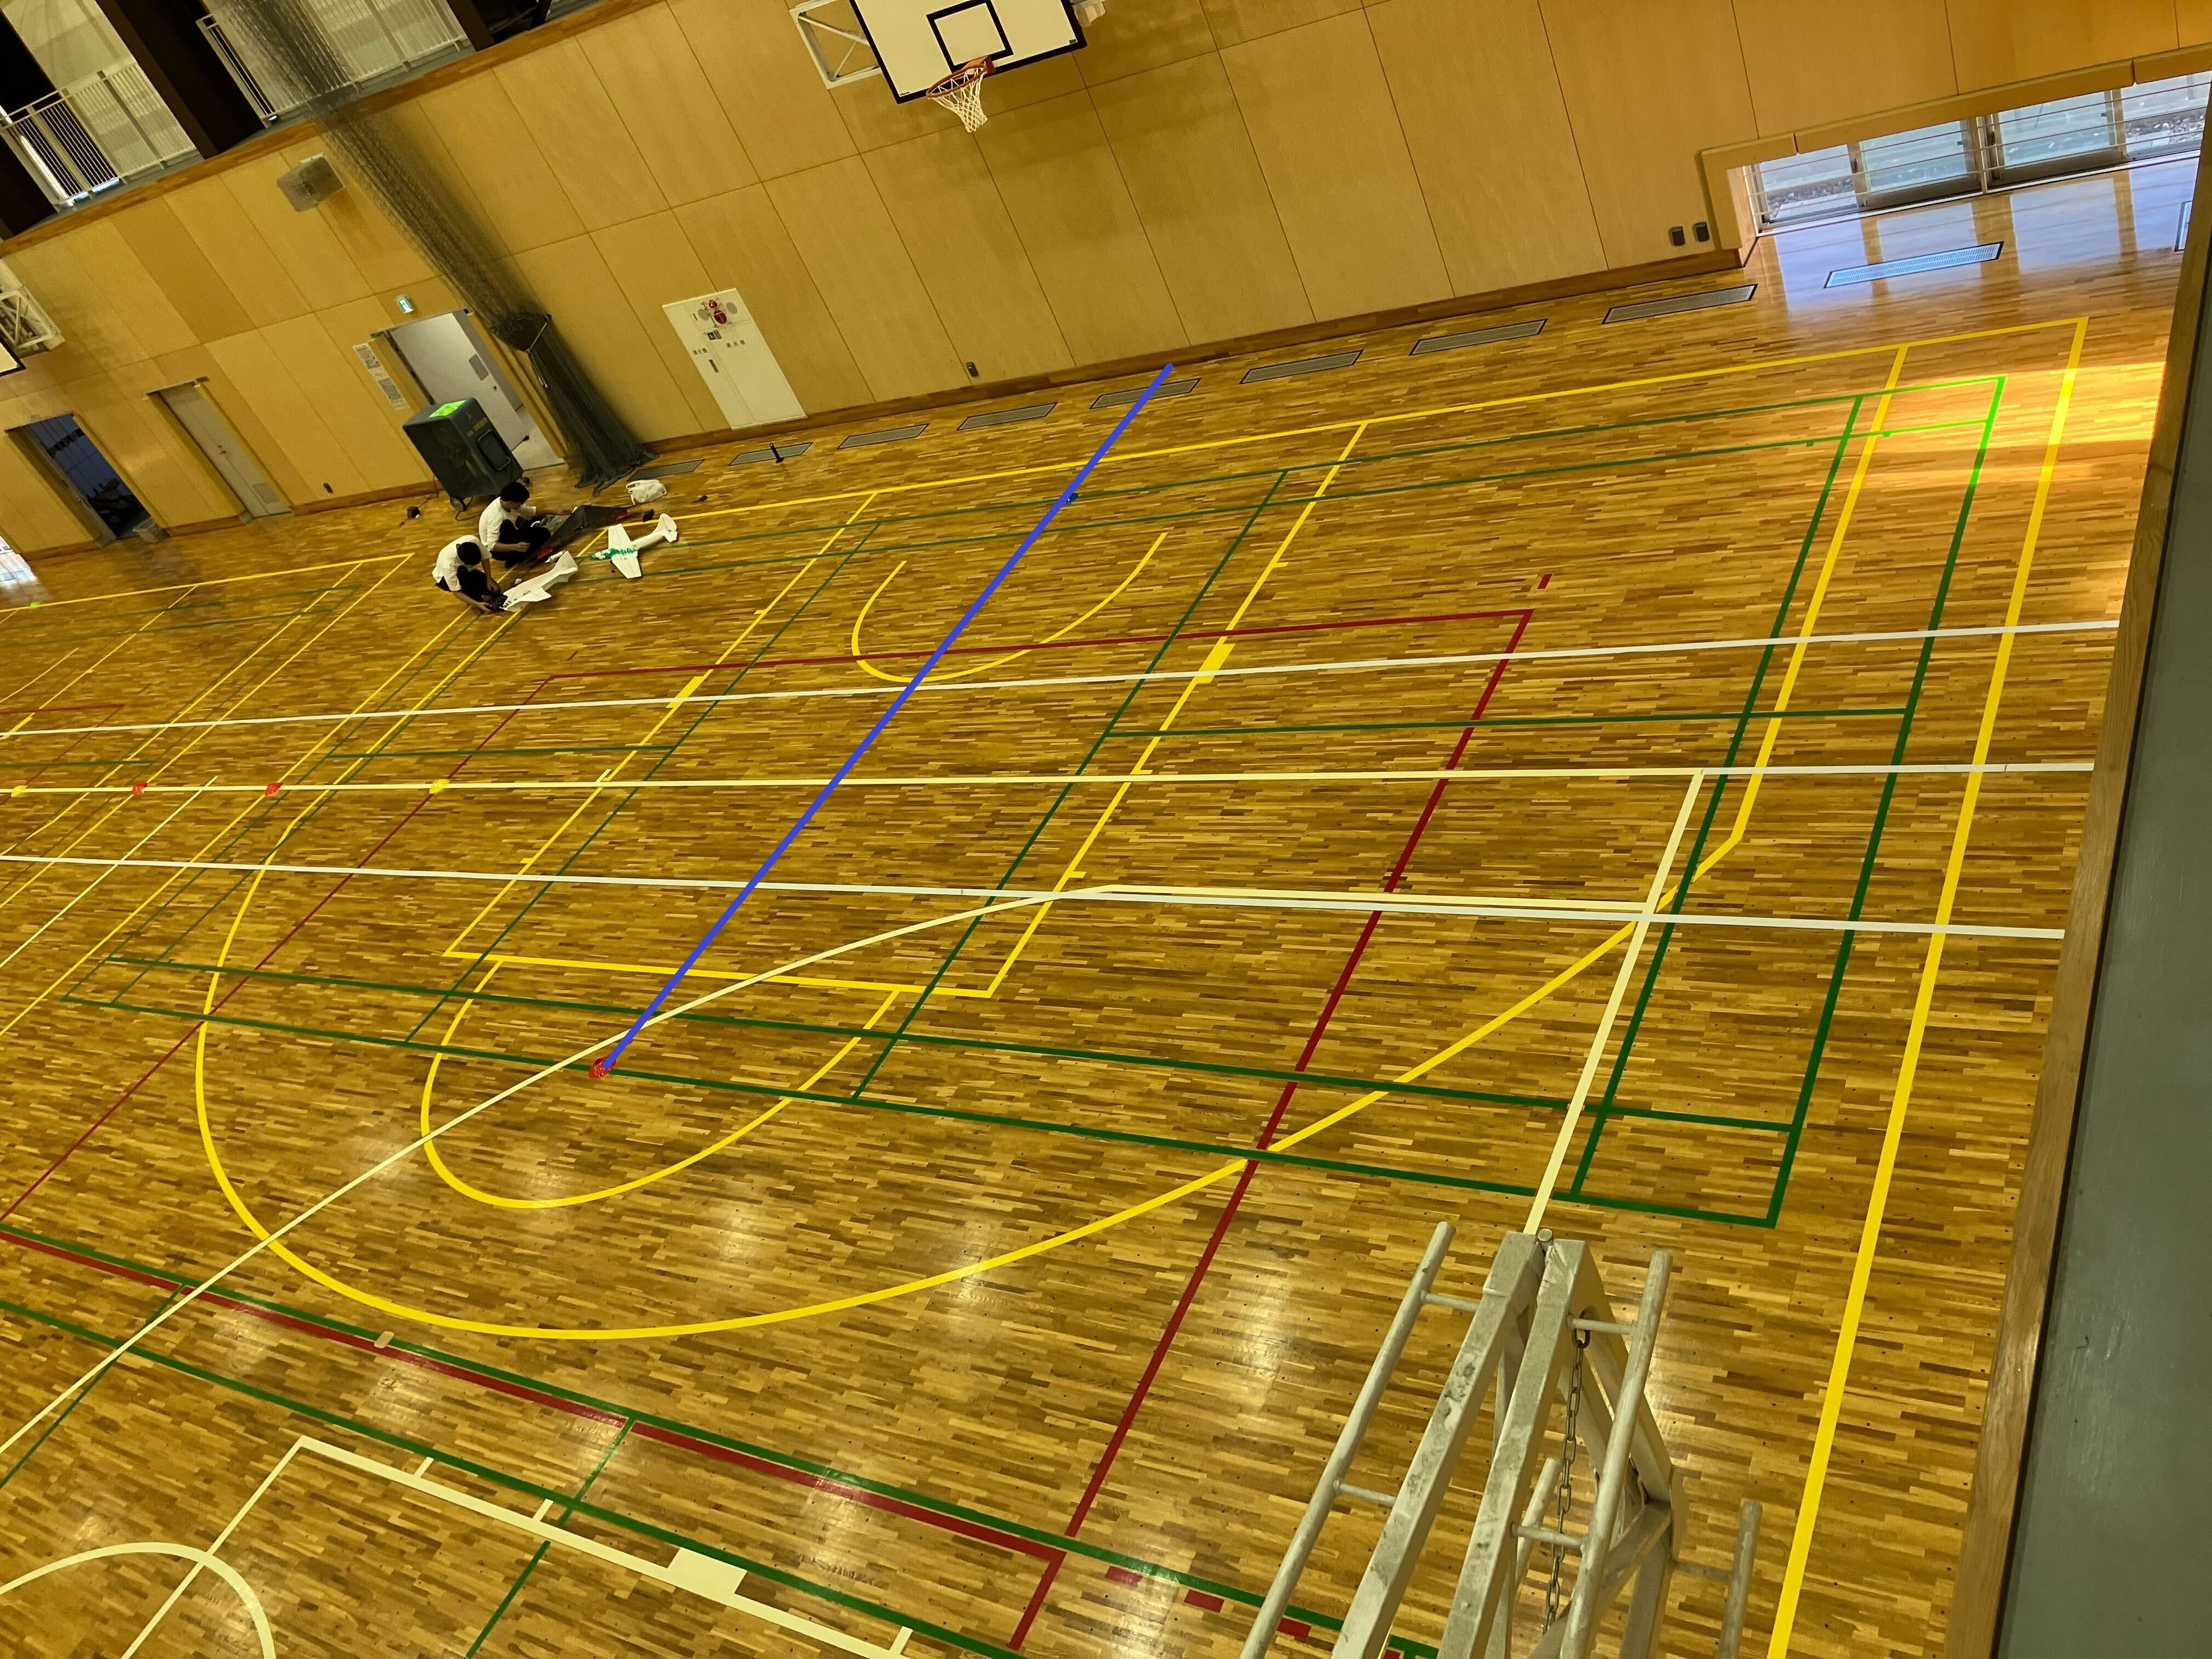
\includegraphics[width=70mm]{plane_poleTurn.jpg}
  \caption{ポール旋回}
  \label{fig::plane::poleTurn}
\end{figure}

\subsubsection{離着陸エリア}
図 \ref{fig::plane::landingZone} に離着陸エリアを示す.
\begin{itemize}
  \item オレンジの斜線部を滑走路とする
  \item 緑の斜線部と滑走路を合わせて離着陸エリアとする
  \item 体育館の壁面は離着陸エリア外とする
\end{itemize}
\begin{figure}[htb]
  \centering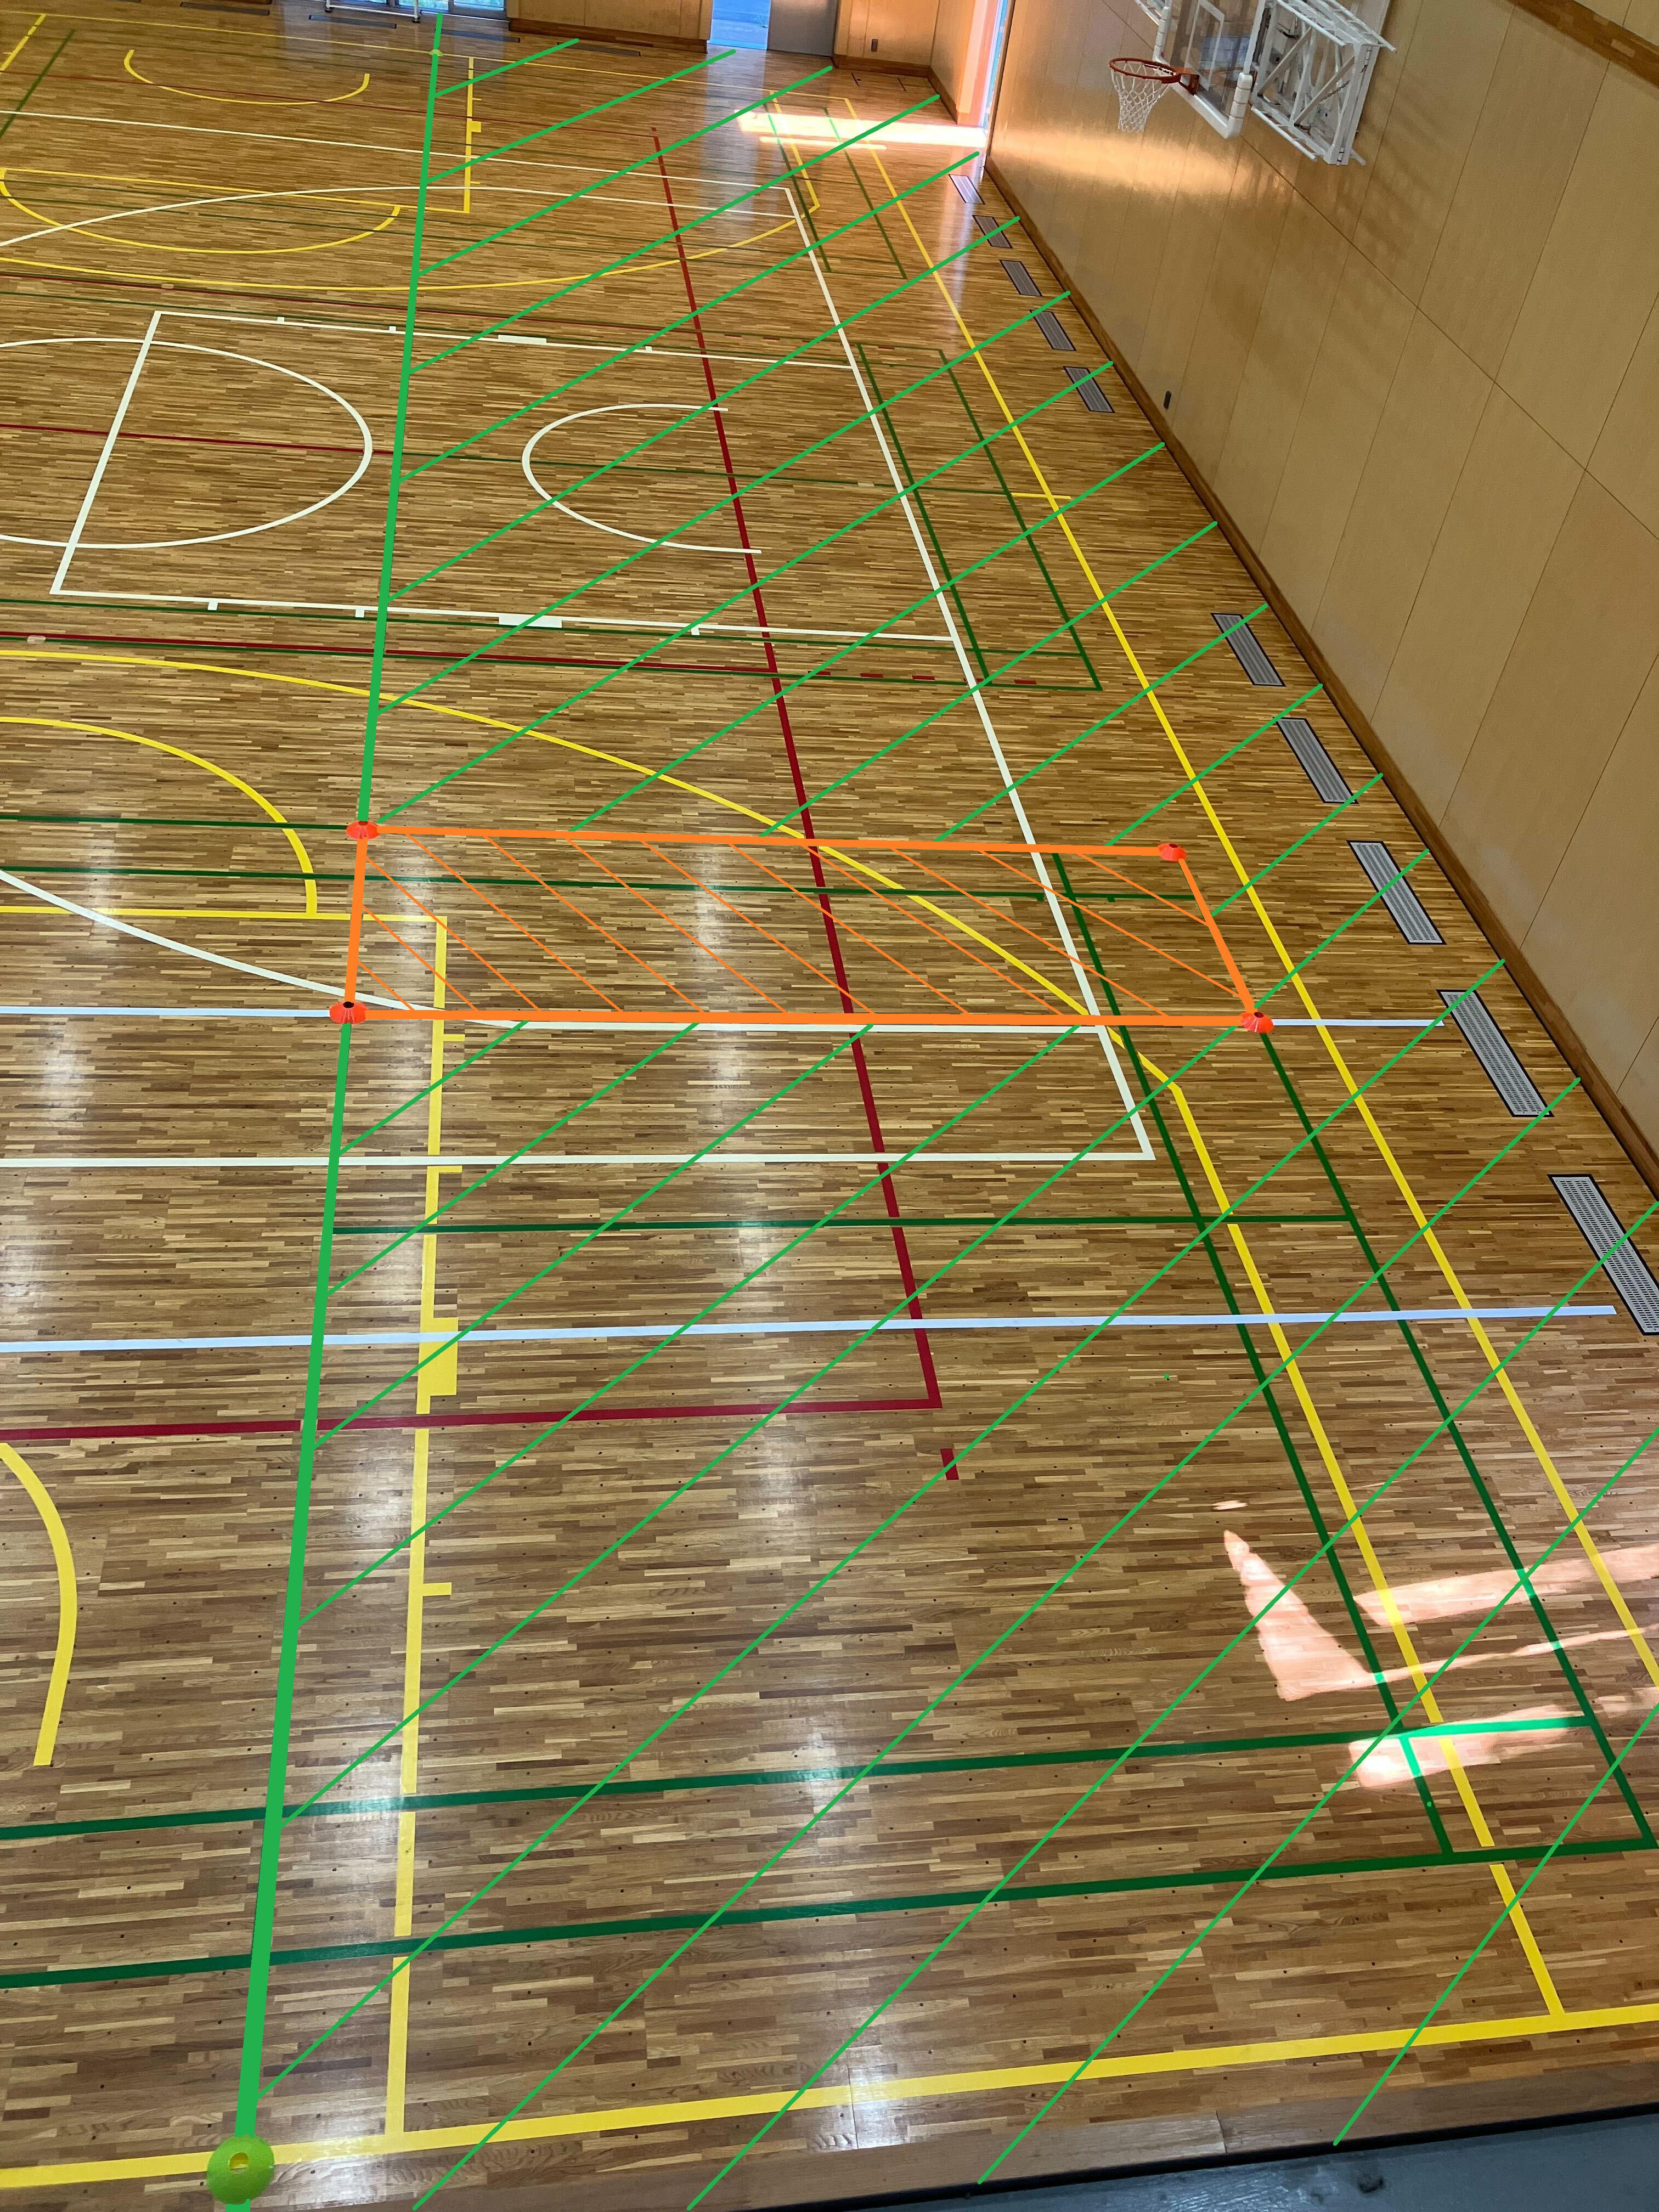
\includegraphics[width = 50mm,angle=90]{./plane_landingZone.jpg}
  \caption{離着陸エリア}
  \label{fig::plane::landingZone}
\end{figure}
\newpage
\section{ミッション(マルチコプター部門)}

\subsection{メインミッション}
\paragraph{成功条件}
\begin{itemize}
\item 物資投下エリアに救援物資を1つ投下すること
\end{itemize}
\paragraph{終了条件}
\begin{itemize}
\item 次のミッションをコールすること
\end{itemize}
\paragraph{得点}
\begin{itemize}
\item メインミッション点 = 時間点+投下点+回収点
\item 時間点 = 20×(60-計測時間)
\item 投下点 = 高所物資運搬点 * 個数 + 救援物資(大)運搬点
\item 高所運搬点 = 200
\item 救援物資(大)運搬点 = 400
\item 回収点 = 400
\item 高所運搬点は高所運搬台に入れた個数に応じて加点する
\item 回収点は救援物資(大)の回収に成功したときに与えられる
\item 投下点は競技終了時の救援物資の位置で確定する
\item 計測時間は競技開始からメインミッションの終了条件を満たすまでの時間とする
\end{itemize}
\paragraph{付記}
\begin{itemize}
\item 救援物資の持ち込みは4個まで認める
\item 4個の救援物資のうち1つを救援物資(大)にすることができる
\item 救援物資(大)は競技開始前に投下エリアの中央に置くこと
\item 投下は,送信機などによる手動操作によって行うのではなく,なんらかの自動装置による制御にて行うこと
\item 大会前の審査を通じて,投下装置の確認ならびに追加や修正を指示することがある
\item 手動操作による投下は得点の対象外とする
\item 高所物資運搬台の中には発行する赤外線投光器が設置される
\item 投下点は高所物資運搬台が倒れていない場合に与えられる
\item 投下点は高所物資運搬台の内部に存在するものが対象となる
\item 競技開始後,救援物資は操縦者もしくは補助員が取り付けることができる.救援物資(大)は操縦者および補助員が取り付けることができない.
\end{itemize}

\subsection{サブミッション}
サブミッションの一覧は以下の通り.
\begin{itemize}
\item ホバリング
\item 大型貨物運搬
\item 8の字飛行
\item 耐故障制御
\item ユニークミッション
\item 帰還
\end{itemize}

\subsubsection{ホバリング}
\paragraph{成功条件}
\begin{itemize}
  \item ホバリングを10秒以上維持すること
\end{itemize}
\paragraph{終了条件}
\begin{itemize}
  \item 次のミッションがコールされること
  \item 成功条件を満たすこと
\end{itemize}
\paragraph{得点}
\begin{itemize}
  \item ホバリング点 = 100
\end{itemize}

\subsubsection{大型貨物運搬}
\paragraph{成功条件}
\begin{itemize}
  \item 離着陸エリアの大型貨物着陸位置に大型貨物が静止すること
  \item 糸の接続状態を保ったまま離着陸エリアに機体が静止すること
\end{itemize}
\paragraph{終了条件}
\begin{itemize}
  \item 次のミッションがコールされること
  \item 成功条件を満たすこと
  \item 大型貨物がフィールドに設置されたものに接触すること
  \item 大型貨物が切り離されること
\end{itemize}
\paragraph{得点}
\begin{itemize}
  \item 大型貨物運搬点 = 運搬点(600点)+ 着陸点(400点)
  \item 運搬点は大型貨物着陸位置に大型貨物が静止し,離着陸エリア内に機体が着陸静止したときに与えられる
  \item 着陸点はバーティポート内に機体が着陸したときに与えられる
\end{itemize}

\subsubsection{8の字飛行}
\paragraph{成功条件}
\begin{itemize}
\item 8の字飛行を行うこと
\item ラインA→ラインB→ラインA→ラインB→ラインAの順に通過すること\newline
このとき2本あるラインBをそれぞれ1回通過すること
\end{itemize}
\paragraph{終了条件}
\begin{itemize}
\item 次のミッションがコールされること
\item 成功条件を満たすこと
\end{itemize}
\paragraph{得点}
\begin{itemize}
\item 8の字飛行点 = 400
\end{itemize}

\subsubsection{耐故障制御}
\paragraph{成功条件}
\begin{itemize}
  \item 動力用モーターが1発以上停止した状態で4秒以上、機体が接地せずに滞空すること
\end{itemize}
\paragraph{終了条件}
\begin{itemize}
  \item 次のミッションがコールされること
  \item ミッション中に機体が接地すること
\end{itemize}
\paragraph{得点}
\begin{itemize}
  \item 滞空時間を「パワーオフ」から「パワーオン」のコールまでの秒数とする
  \item 滞空時間の条件を8秒とする
  \item 耐故障制御点 = 400 + 100$\times$滞空時間
\end{itemize}

\subsubsection{ユニークミッション}
成功条件や終了条件は後日決定される.
得点は1~1000点の間で設定される.

\subsubsection{帰還}
\paragraph{成功条件}
\begin{itemize}
\item 離着陸エリア内で接地して機体が完全に静止すること
\end{itemize}
\paragraph{終了条件}
\begin{itemize}
\item 機体が静止すること
\end{itemize}
\paragraph{得点}
\begin{itemize}
\item 帰還点 = 着陸点(100点)+バーティポート内着陸点(100点)
\item 離着陸エリア内に接地した場合,着陸点として100点を加算する
\item バーティポート内で着陸静止した場合,バーティポート内着陸点として100点を加算する
\end{itemize}
\paragraph{付記}
\begin{itemize}
\item 帰還が終了したとき競技を終了とする
\end{itemize}


\subsection{フィールド}
\subsubsection{物資投下エリア}
物資投下エリア \ref{fig::multicopter::dropArea} に示す.
黄色の枠の内側が物資投下エリアである.
高所物資運搬台は写真と同様の位置に配置する.
当日のフィールドでは図と同じ位置にマーカーを置き物資投下エリアの基準とする.
\begin{figure}[ht]
  \centering\includegraphics[width = 50mm,angle=90]{./multicopter_dropArea.png}
  \caption{物資投下エリア}
  \label{fig::multicopter::dropArea}
\end{figure}

\newpage
\subsubsection{8の字飛行用のポール}
8の字飛行で使用するポール周辺のフィールド図を図 \ref{fig::multicopter::poleTurn} に示す.
2本のポールの間(オレンジ線)をラインAとする.
ポールの外側(青線)をラインBとする.
\begin{figure}[h]
  \centering\includegraphics[width=70mm]{multicopter_poleTurn.png}
  \caption{8の字飛行用のポール}
  \label{fig::multicopter::poleTurn}
\end{figure}
\end{document}